\chapter{The HH$\rightarrow$4b Analysis}\label{ch:hh4b}

In section \ref{sec:beyond_sm} the importance of measuring the exact form of the Higgs potential was discussed. This thesis concentrates on the $4b$-quark final state to contribute to this effort. The main Higgs pair production modes at the \ac{lhc} are illustrated in Figure \ref{fig:main_production_processes}. The Higgs boson interacts with fermions through Yukawa couplings, as described by equation \ref{eq:yukawa_term}. These couplings are proportional to fermion masses, thus the Higgs boson prefers coupling to heavier particles, such as the top quark or massive vector bosons. All couplings are scaled relative to their \ac{sm} values and are denoted as $\kappa_\mathrm{c} = c/c_\mathrm{sm}$, where a $\kappa_\mathrm{c}$ value of 1 corresponds to the \ac{sm} value for a given coupling $c$.

The first two \ac{ggf} diagrams \ref{fig:main_production_processes}(a) and \ref{fig:main_production_processes}(b) have a cross-section of $\sigma_\text{vbf HH}^\text{SM}=\qty[]{31.05}{fb}$, calculated at a center of mass energy of \qty[]{13}{TeV} at \ac{nnlo} \citep{Grazzini_2018}. In contrast, the \ac{vbf} processes (c), (d) and (e) of figure \ref{fig:main_production_processes} have a production cross-section of
$\sigma_\text{vbf HH}^\text{SM}=\qty[]{1.73}{fb}$ at \ac{nnnlo} \citep{PhysRevD.98.114016}. A characteristic of the \ac{vbf} processes is that the Higgs pair is accompanied by two additional quarks in the final state. This \ac{vbf} cross section is about \qty[]{3e4}{} times smaller than for single Higgs production at the \ac{lhc} $\sigma_\text{H}^\text{SM}=\qty[]{48.58}{pb}$ \citep{de2016arxiv} and underlines the challenge of discovering Higgs pairs.

\begin{figure}
    \centering
    \subfigure[]{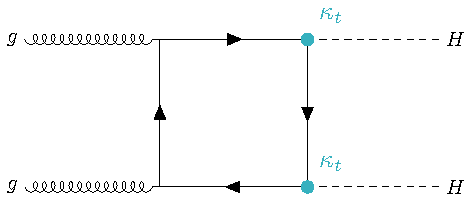
\includegraphics[width=.43\textwidth]{fig_01a}}\hspace{.06\textwidth}
    \subfigure[]{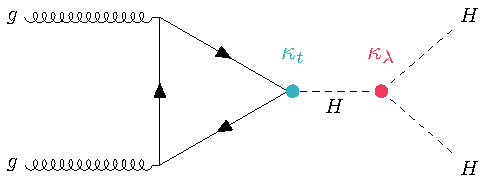
\includegraphics[width=.43\textwidth]{fig_01b}} \\
    \subfigure[]{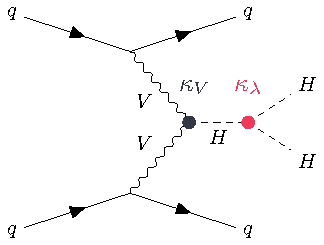
\includegraphics[width=.3\textwidth]{fig_02a}}\hspace{.01\textwidth}
    \subfigure[]{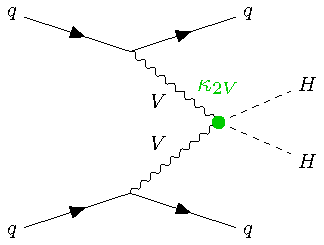
\includegraphics[width=.3\textwidth]{fig_02b}}\hspace{.01\textwidth}
    \subfigure[]{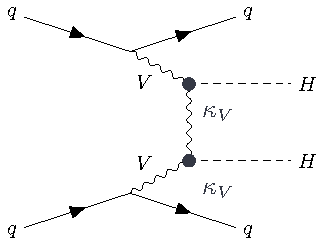
\includegraphics[width=.3\textwidth]{fig_02c}}
    \caption[]{Leading Higgs Pair production processes at the \ac{lhc}. (a), (b) shows \ac{ggf} and (c), (d), (e) \ac{vbf} processes. Adopted from \citep{aad2023search}.}
    \label{fig:main_production_processes}
\end{figure}
% higgs hat keine Ladung whatsoever cannot couple em or qcd 

\begin{figure}
    \centering
    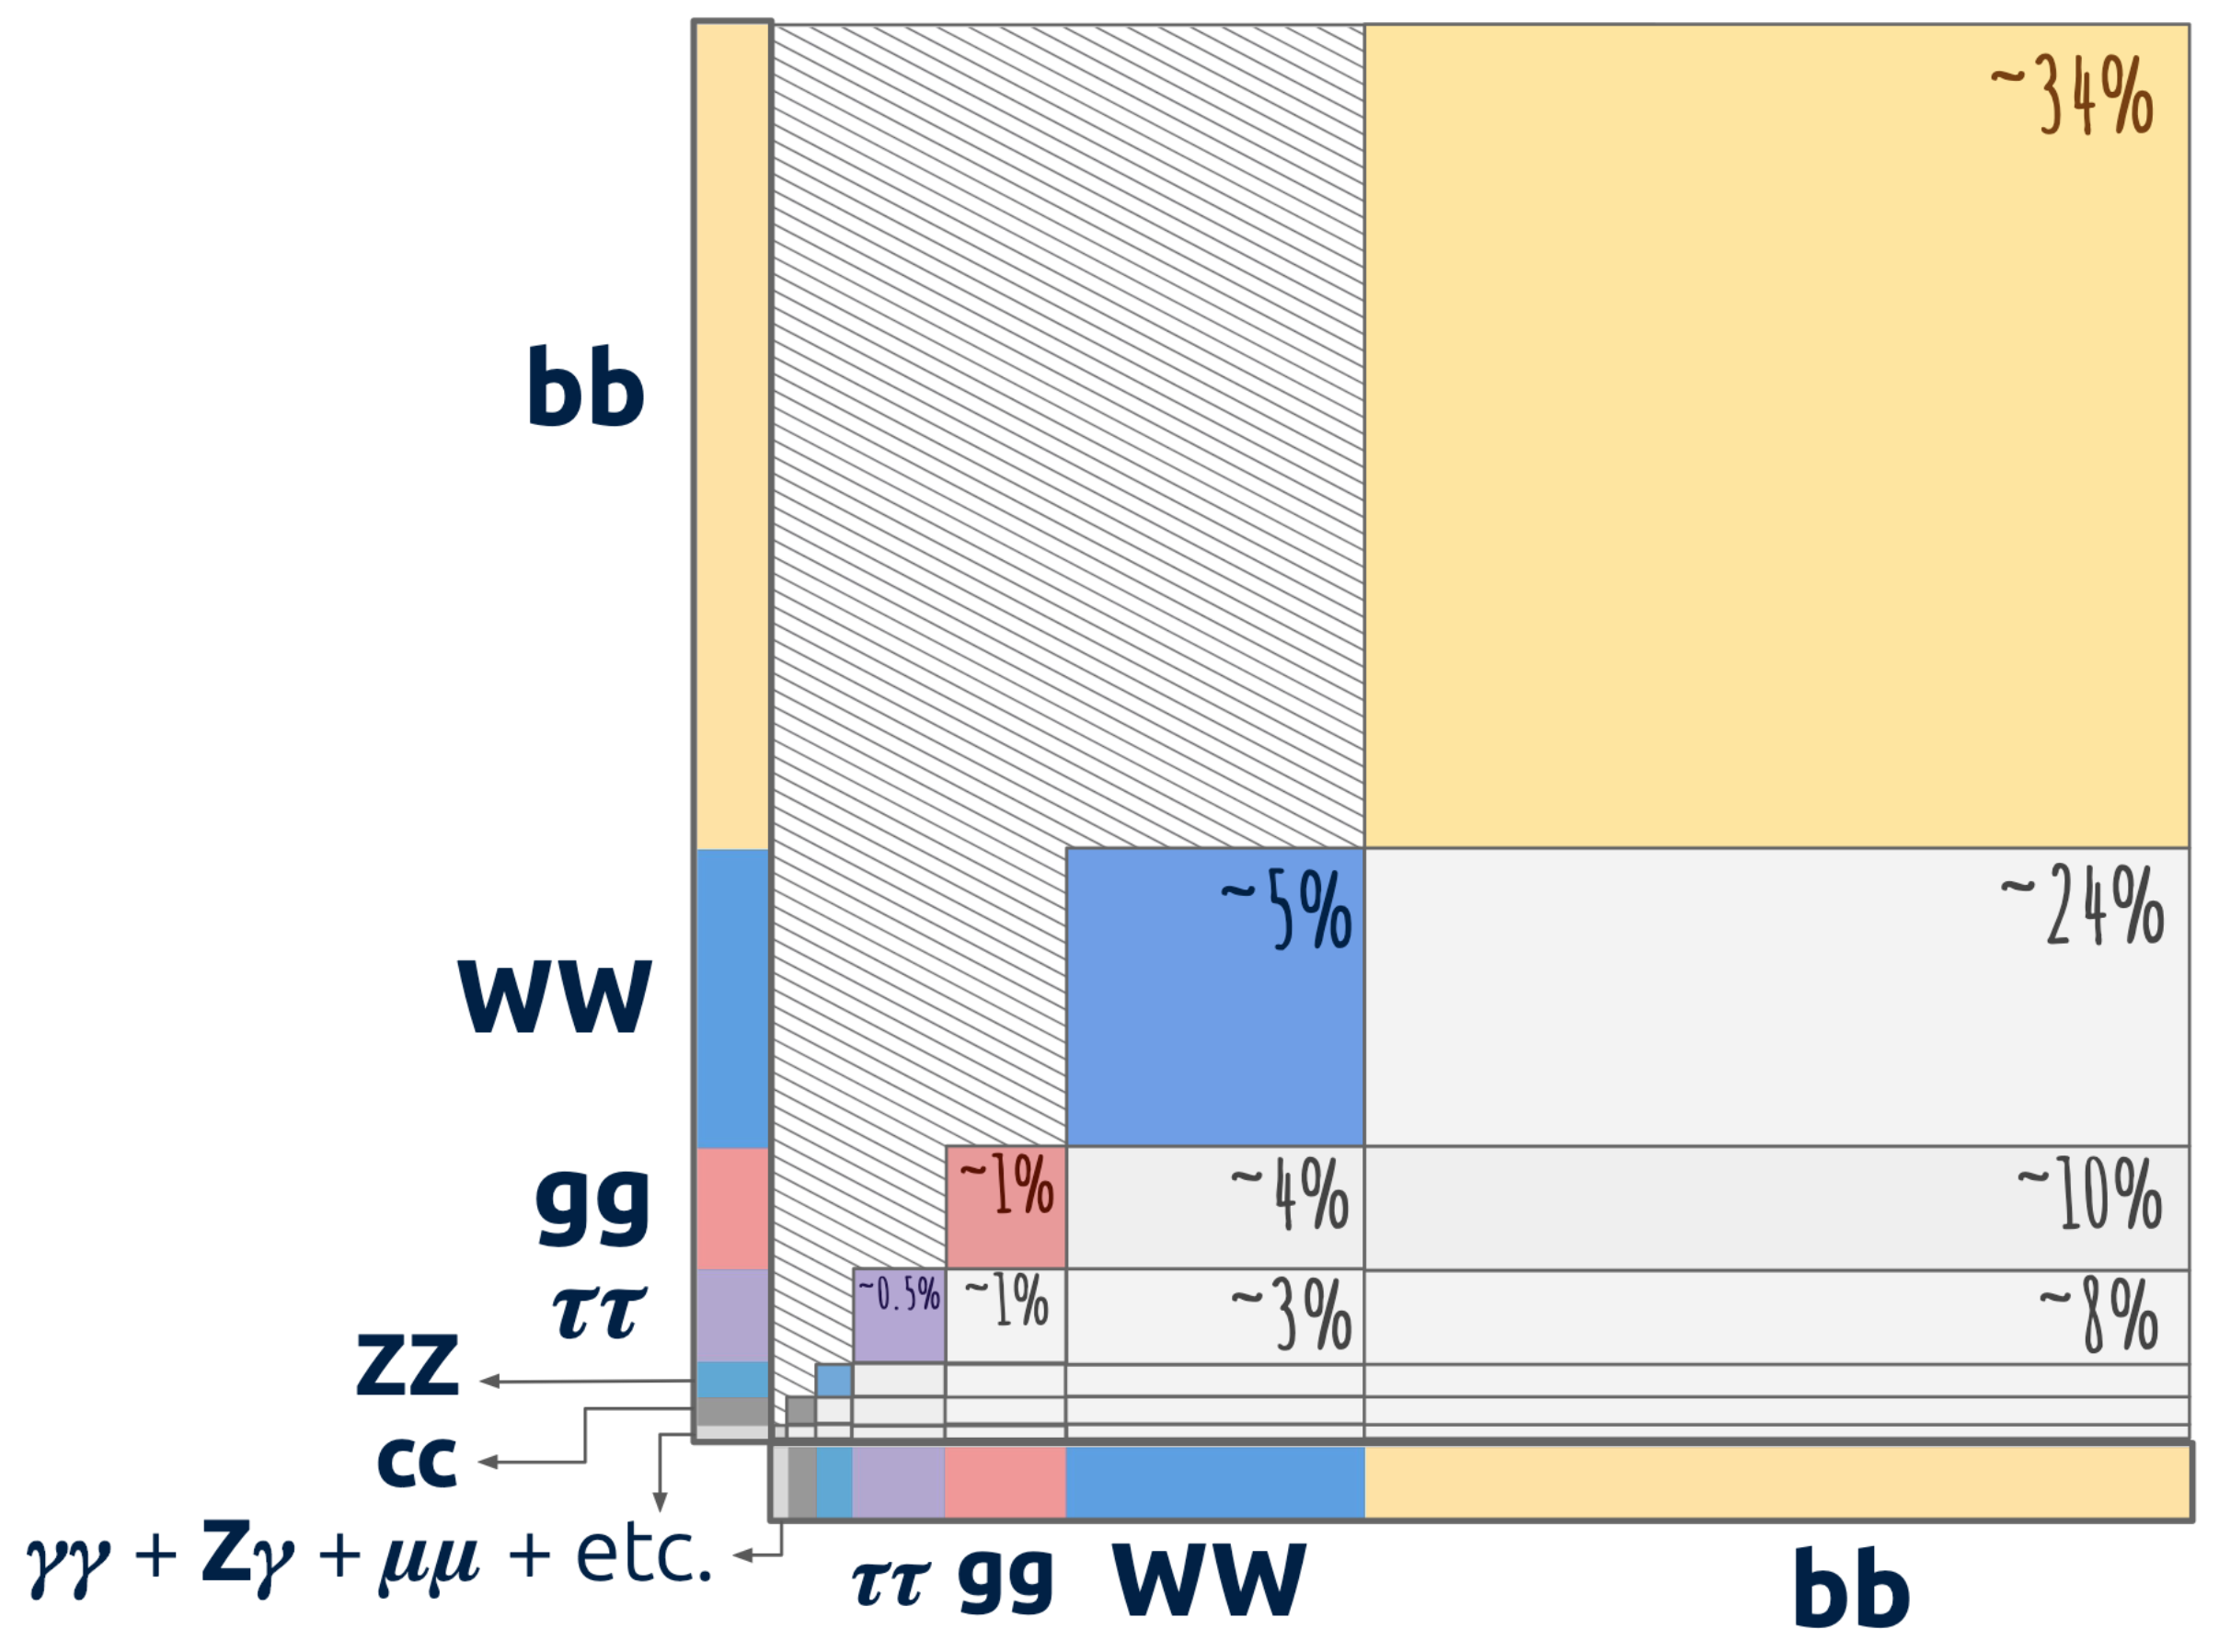
\includegraphics[width=0.7\textwidth]{branching_fraction_hh}
    \caption[]{Contributions of final states represented by area for a pair of Higgs. Adopted from \citep{ATL-COM-PHYS-2020-083}.}
    \label{fig:branching_fraction_hh}
\end{figure}
Figure \ref{fig:branching_fraction_hh} highlights that an interesting channel in the study of Higgs pair production is the final state consisting of four $b$-quarks, with the largest branching fraction amounting to about \qty[]{34}{\percent}. Thus the \ac{sm} \ac{vbf} cross-section is calculated to correspond to the 4b branching ratio by multiplying it with $\mathcal{B}(4b)=0.3392$. As this is a fully hadronic final state a challenge lies in the presence of significant \ac{qcd} backgrounds.

This work focuses on the boosted topology of highly energetic jets which do not allow reconstruction of $b$-jets individually but rather of final states consisting of large-$R$ jets encapsulating two collimated $b$-jets inside. This approach substantially reduces \ac{qcd} backgrounds, as highly energetic jets are more likely to originate from heavy particles like $b$-quarks. Moreover, events with jets of large transverse momentum provide distinct signatures, making events easier to triggering on. Although representing a comparatively clean signal, such events are rare and thus have limited statistical power. While other decay signatures might be more advantageous for the discovery of the Higgs pair production process the value of this selection lies in proving the existence of the \ktwov coupling shown in figure \ref{fig:main_production_processes}(d) to which it is particularly sensitive.

The low cross-section for this process is due to the fact that diagrams (d) and (e) in Figure \ref{fig:main_production_processes} interfere destructively for \ac{sm} values \citep{bishara2017higgs}. Conversely, when $\ktwov$ deviates from \ac{sm} values, the production cross-section increases significantly, with $\sigma_{\ktwov=0}\approx 20\times \sigma_{\ktwov=1}$ and the decay products exhibit much larger transverse momentum, as illustrated in Figure \ref{fig:kappa_2v_variations_mhh}.
\begin{figure}
    \centering
    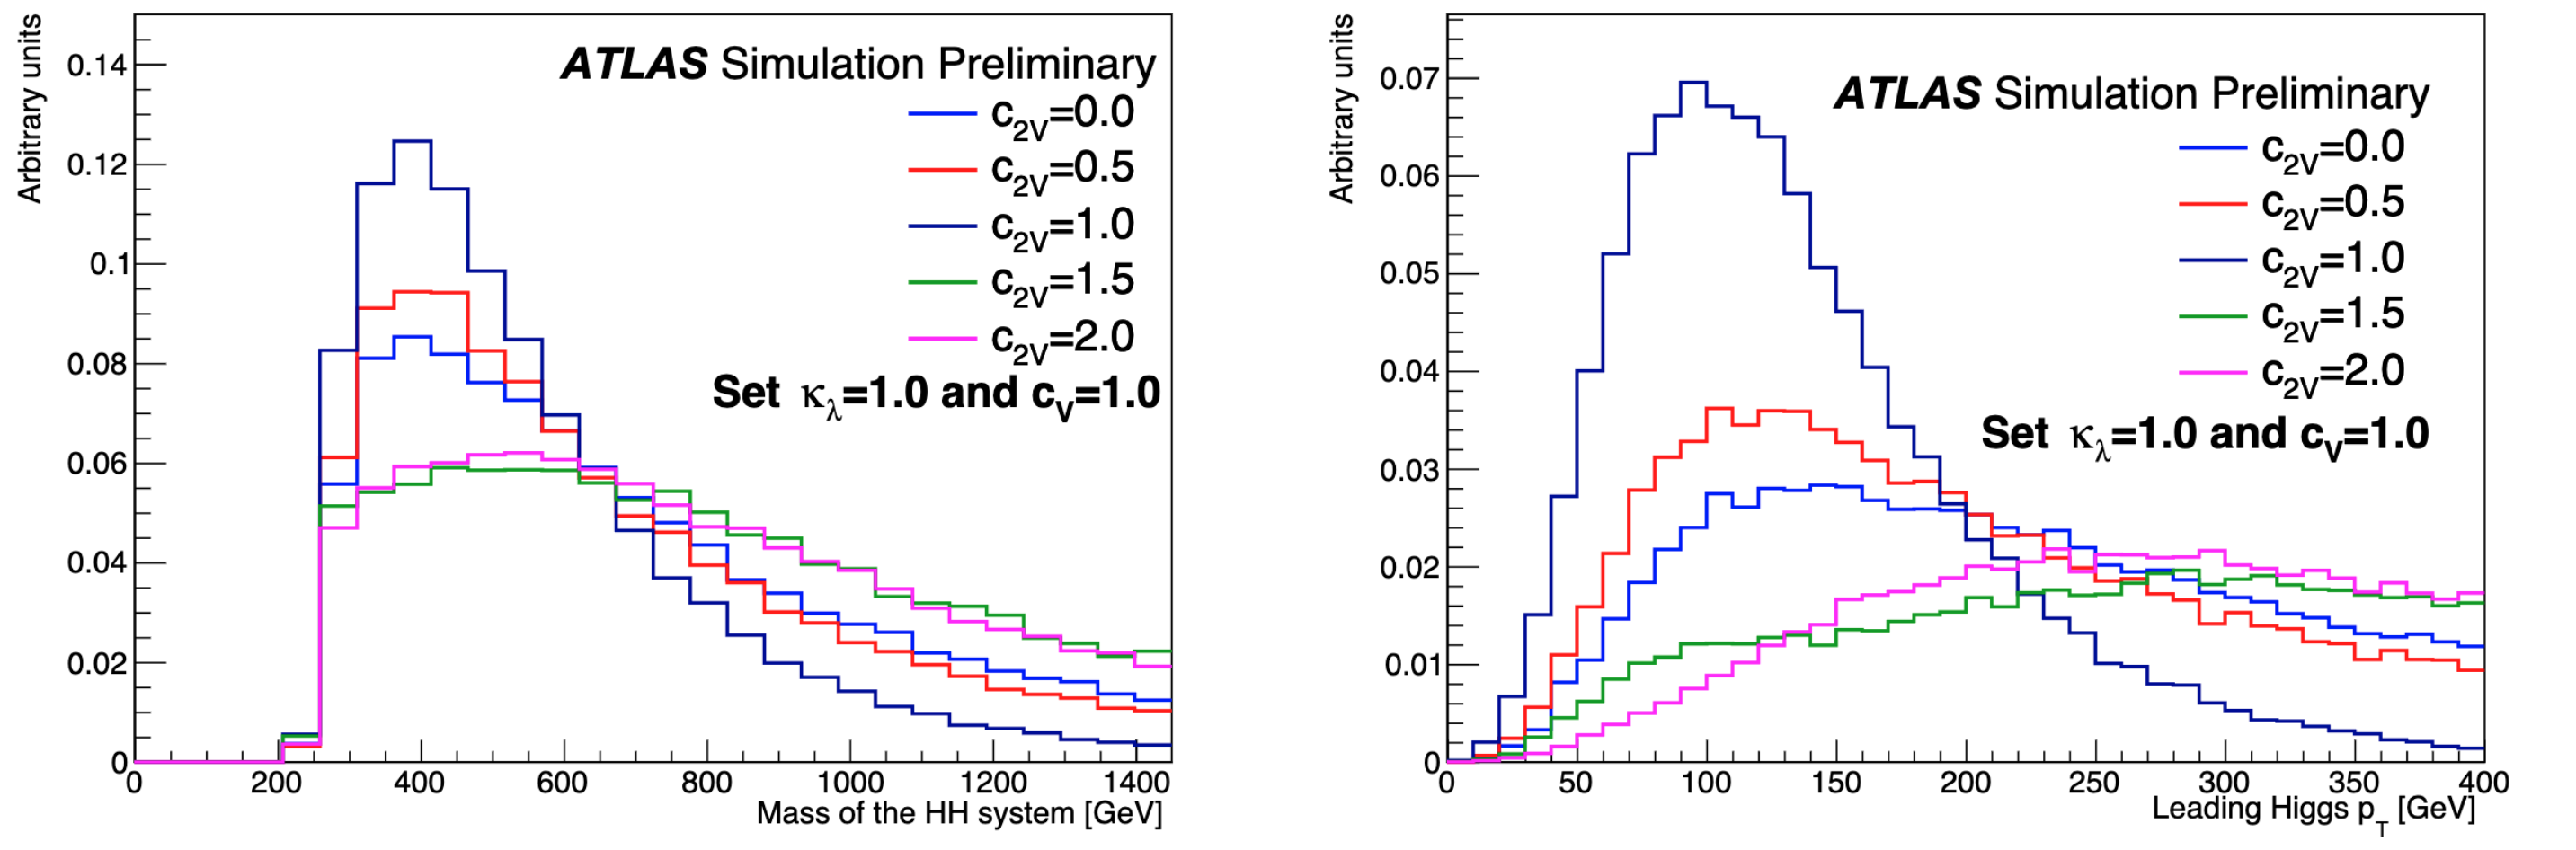
\includegraphics[width=1\textwidth]{kappa_2v_variations_mhh}
    \caption[]{Invariant mass of the Higgs pair system and the leading Higgs candidate jet \pt  reconstructed from simulation for different \ktwov. Adopted from \citep{ATL-PHYS-PUB-2019-007}.}
    \label{fig:kappa_2v_variations_mhh}
\end{figure}

\section{Data And Monte Carlo Simulation}\label{sec:mc_simulation}
This analysis uses the full run 2 data taken by \ac{atlas} between 2015 and 2018. The dataset contains \qty[]{140.1}{fb^{-1}} of data good for physics at a center of mass energy of \qty[]{13}{TeV} \citep{DAPR-2021-01}.

\ac{mc} generation in \ac{atlas} typically involves three steps. At first at parton level the matrix element of the process of interest is stochastically simulated. In this analysis \textsc{MadGraph} (v.2.7.3p3.atlas6) \citep{alwall2014automated} is used for this. The cross sectional calculation for proton-proton collisions relies on the factorization theorem \citep{halzen1984introductory} which states that contributions from partons participating in the hard scatter event can be factorized. Further partons cannot be observed individually since the approximation of the perturbation ansatz of section \ref{sec:qft} breaks down for low energy scales $\mu^2$ as described in section \ref{sec:renormalization}. This is the energy scale for which the approximation would need to hold to describe the partons inside a proton. However parton densities can be studied within \ac{qcd} using the DGLAP equations \citep{thomson2013modern}. Similar to renormalization, a scaling behavior can be derived from these equations that allows to derive an estimate of the \acp{pdf} by measuring it at some factorization scale $\mu_F^2$ in order to extrapolate it to another. Figure \ref{fig:pdf} exemplifies this for two energy scales from the \textsc{NNPDF3.0nlo} \ac{pdf} set used in this analysis.
\begin{figure}
    \centering
    \subfigure[]{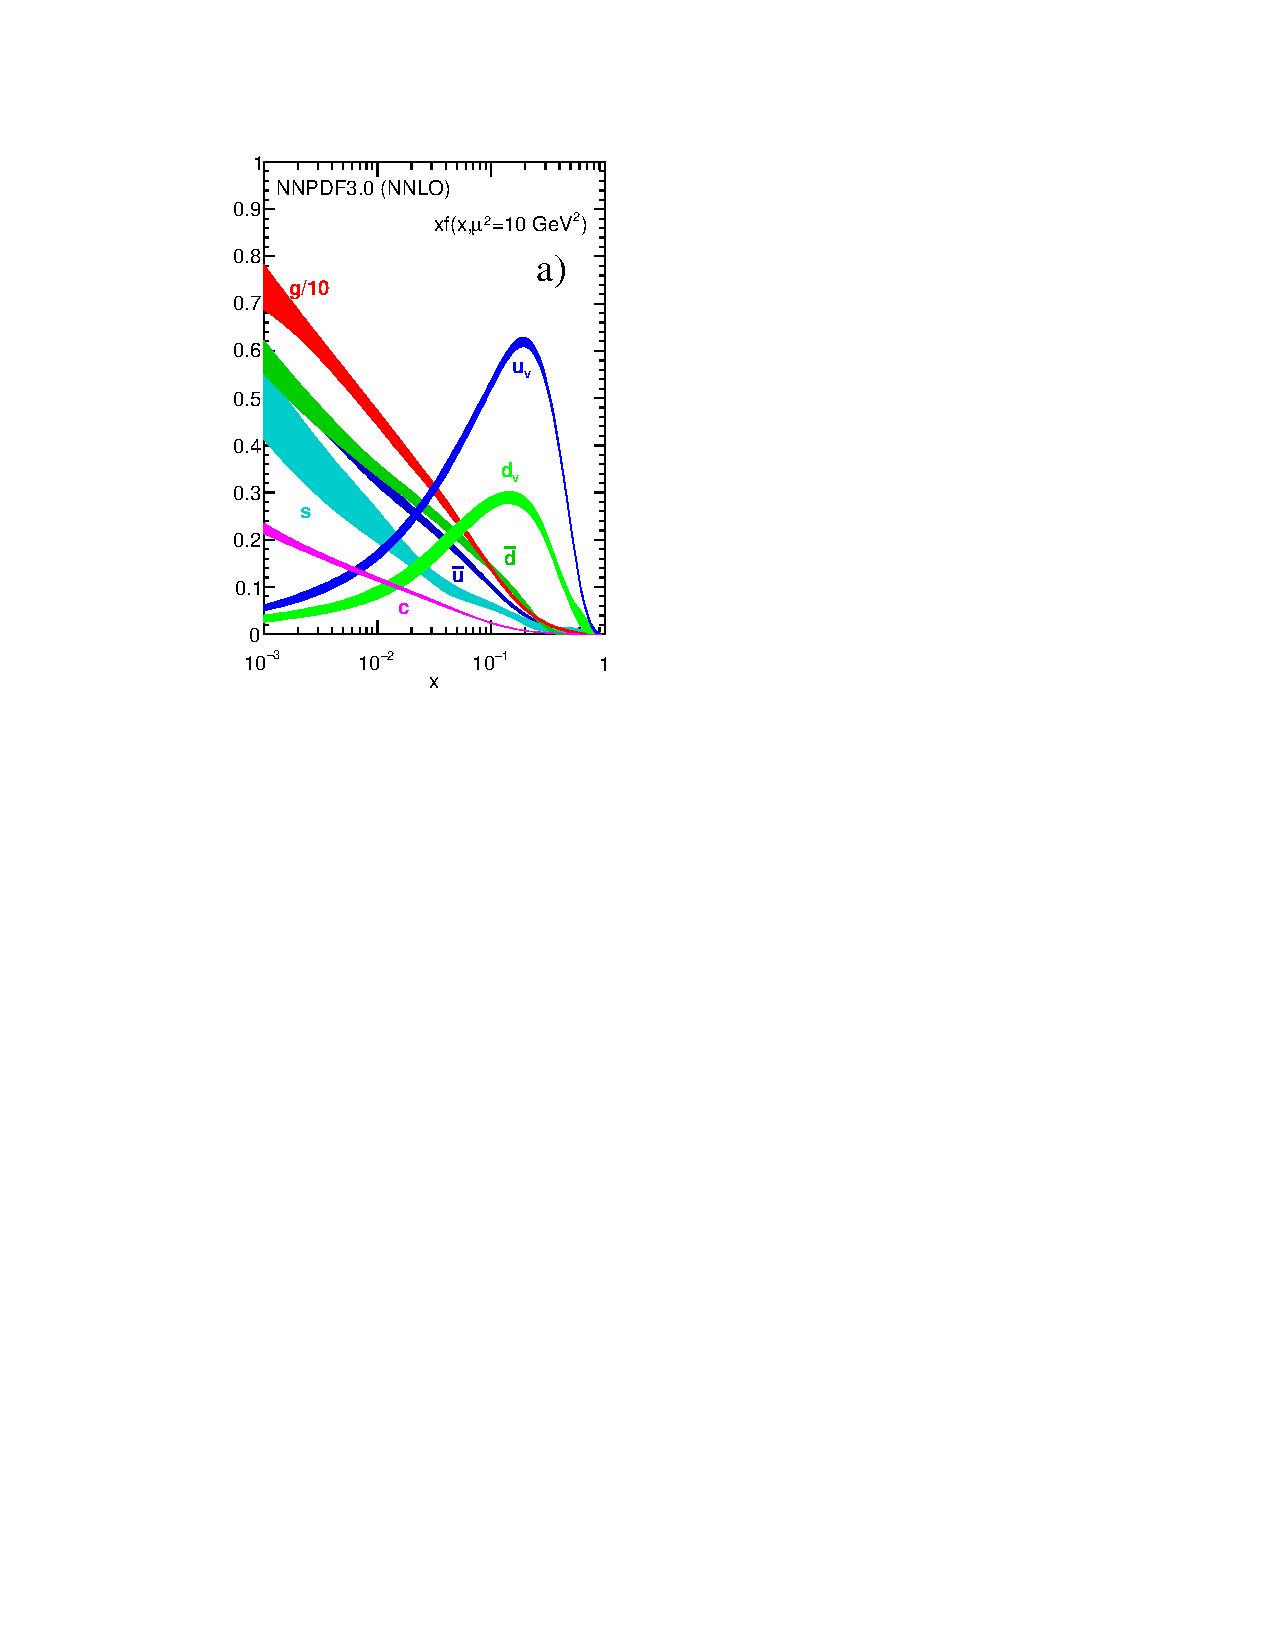
\includegraphics[width=.47\textwidth]{NNPDF-10}}
    \subfigure[]{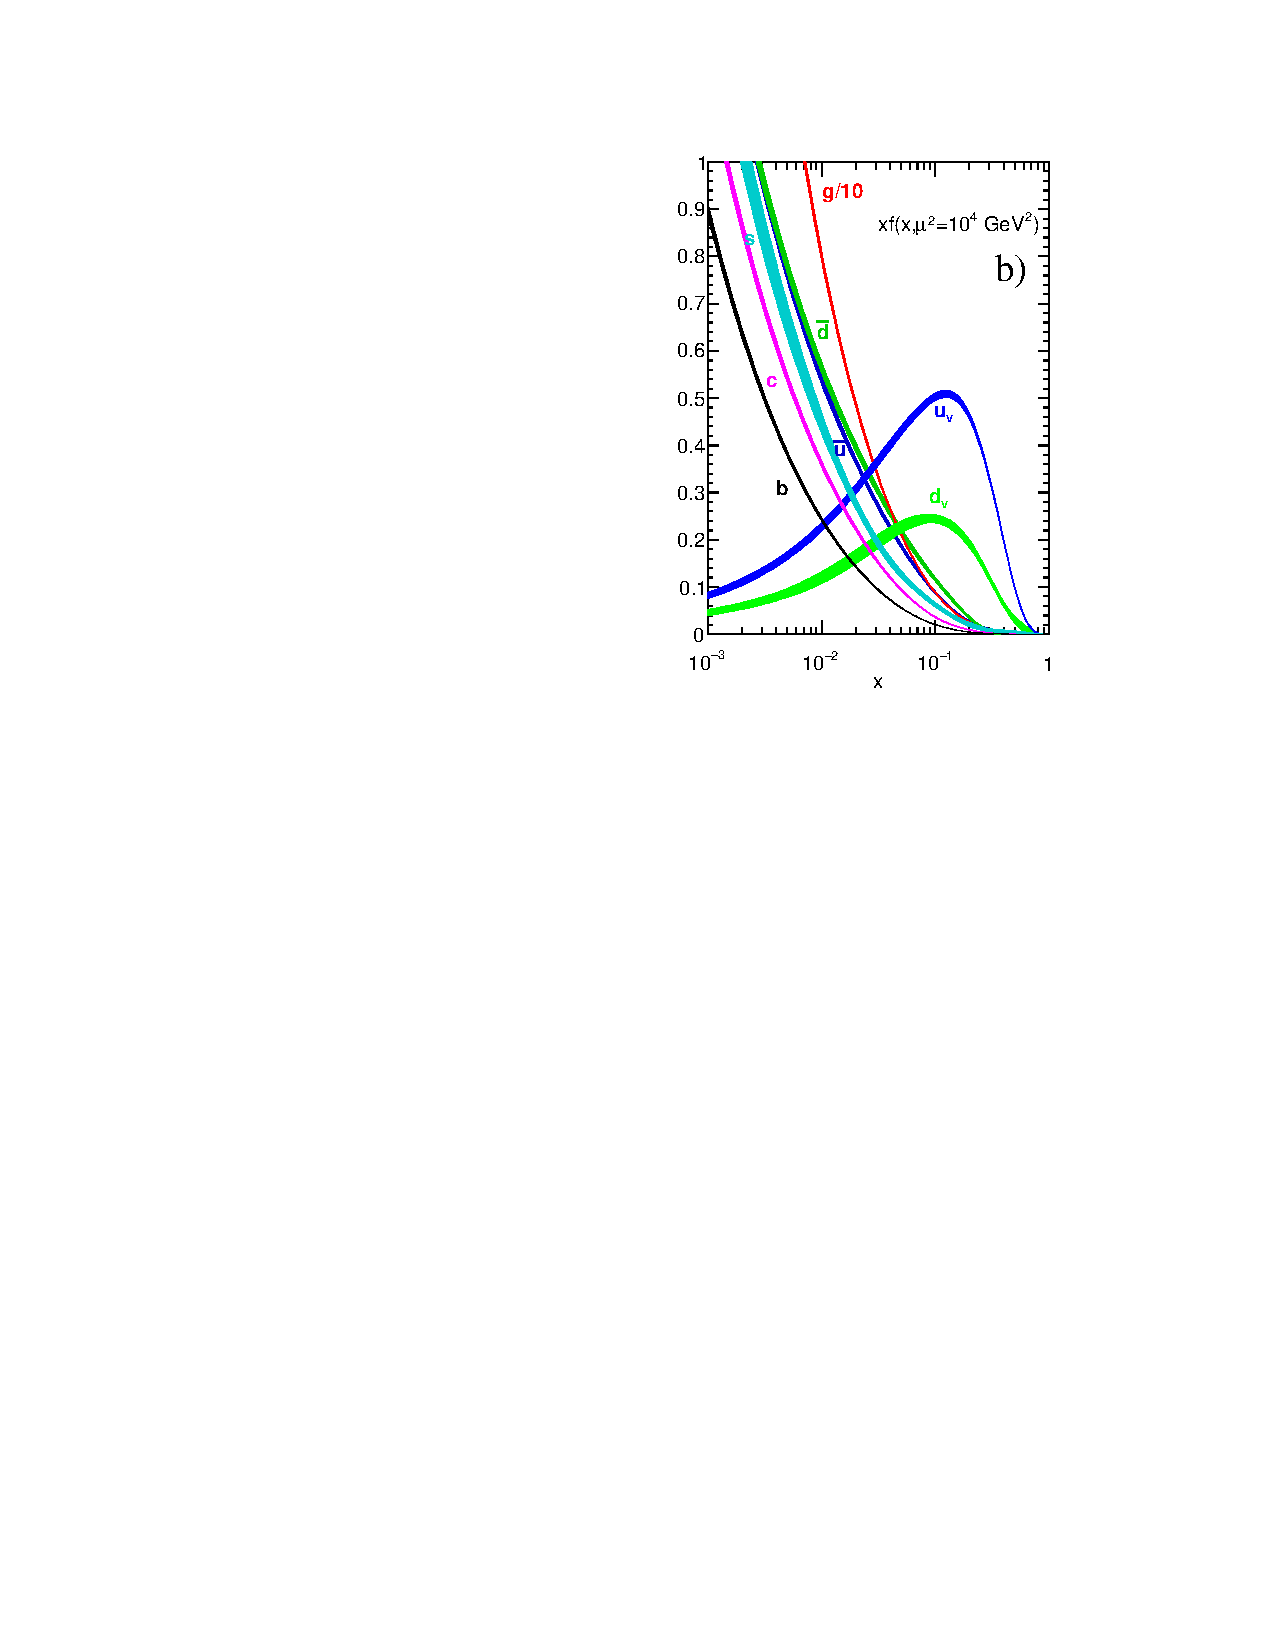
\includegraphics[width=.47\textwidth]{NNPDF-10000}}
    \caption[]{\textsc{NNPDF3.0nlo} parton distribution functions for two different factorization scales (a) $\mu_F^2=$\qty{10}{GeV}$^2$ and (b) $\mu_F^2=$\qty{10}{TeV}$^2$ against the momentum fraction $x$ of the particle. Hence at lower energies gluons and heavier quarks have a larger probability to participate in the interaction. Adopted from \citep{PhysRevD.98.030001}.}
    \label{fig:pdf}
\end{figure}
Thus for hadrons $A,B$ containing partons $a_i,b_i$ and their respective \acp{pdf} $f_{a}^A$ and $f_{a}^B$, dependent on the parton's momentum fraction $x$ and factorization scale $\mu_F^2$, the cross-section of a process $A,B\rightarrow X$ reads
\begin{equation}
    \sigma_{A,B\rightarrow X} = \sum_{a,b} \int_0^1 \text{d}x_1\text{d}x_2 f_a^A(x_1,\mu_F^2) f_b^B(x_2,\mu_F^2) \hat{\sigma}_{a,b\rightarrow X}(\alpha_s(\mu_R^2),\mu_R^2).
\end{equation}
$\hat{\sigma}_{a,b\rightarrow X}$ is the perturbatively calculable part and depends on the strong coupling $\alpha_S$ and renormalization scale $\mu_R^2$.

In a second step the parton shower evolution including hadronization and initial and final state radiation is simulated with \textsc{Pythia8} \citep{Sjostrand:2014zea}. Figure \ref{fig:parton_shower} illustrates this process.
\begin{figure}[]
    \centering
    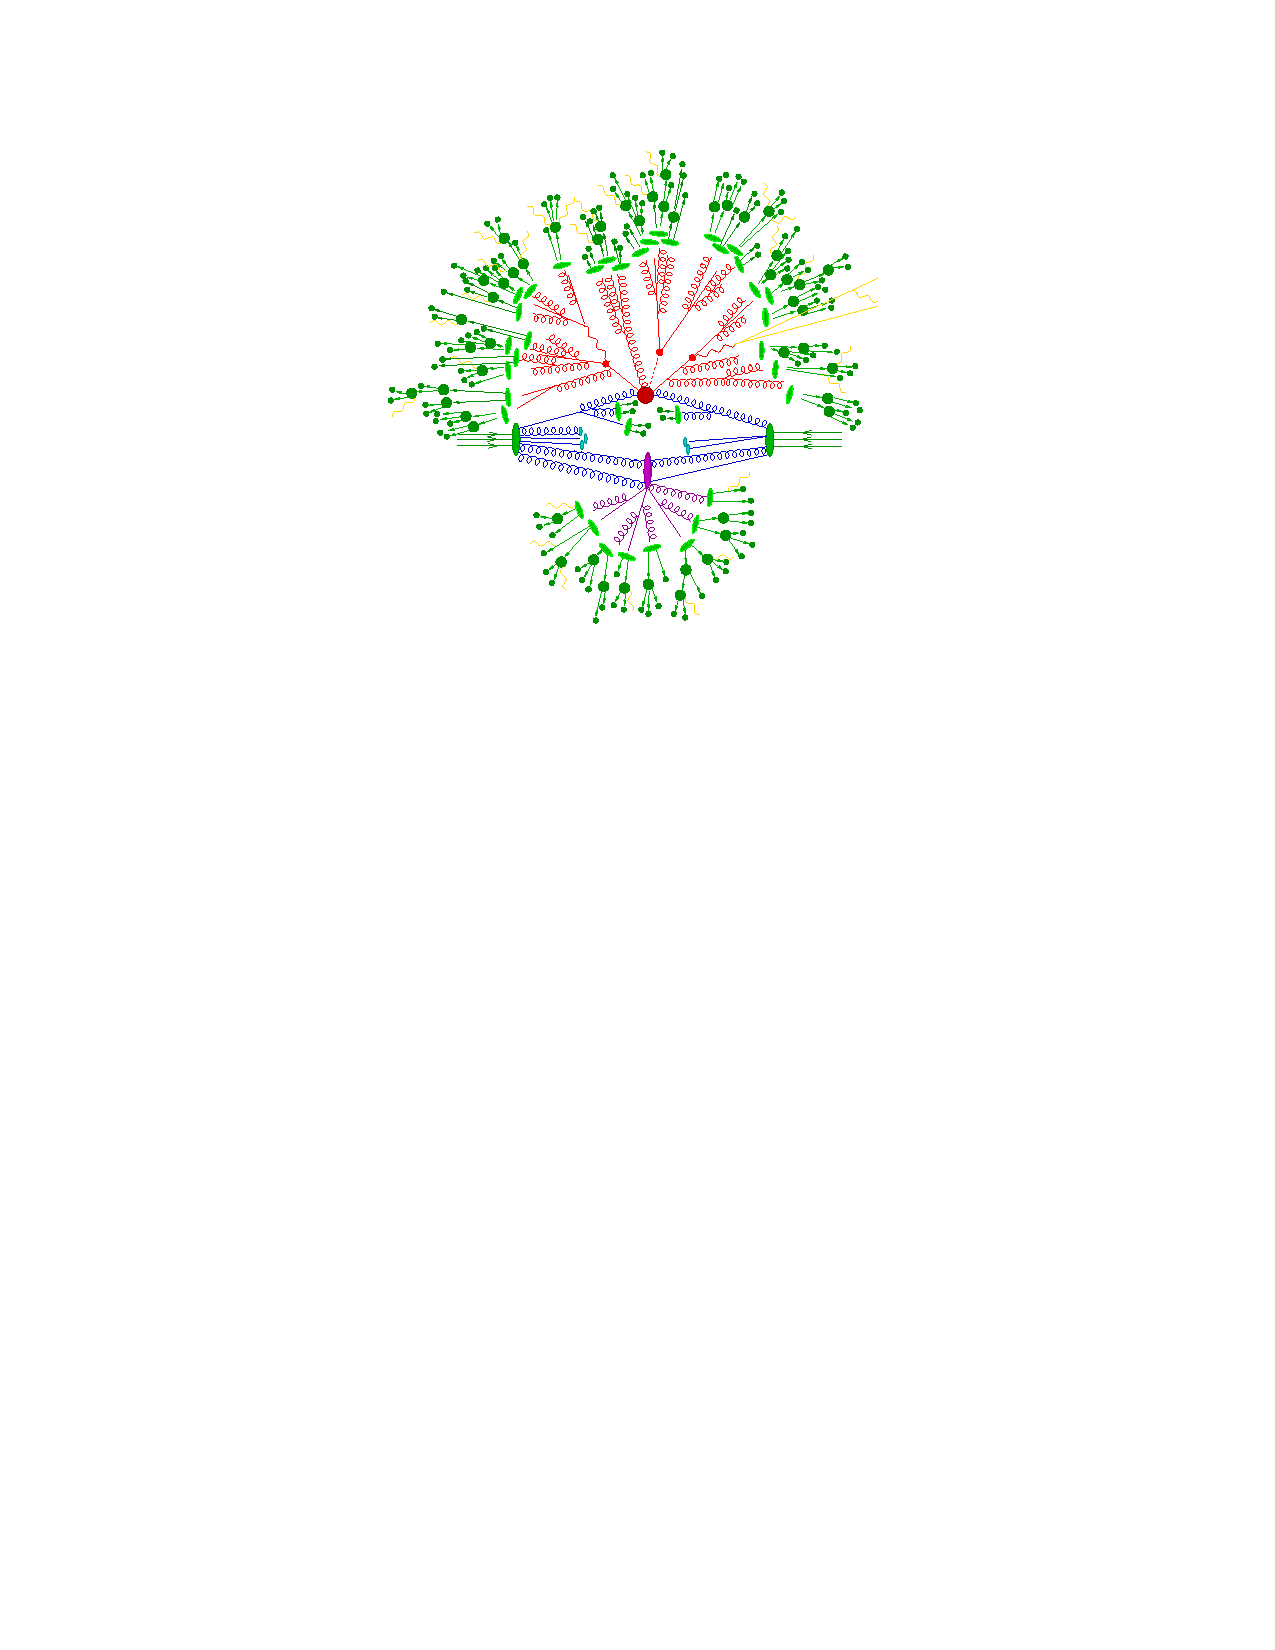
\includegraphics[width=.75\textwidth]{parton-shower}
    \caption{Simulation of an evolution of a proton proton collision: The red circle at the center is the hard collision and the purple oval a secondary hard scatter event. Both are surrounded by a tree-like structure of \ac{qcd} bremsstrahlung interactions simulated with a parton shower. Light green represent hadrons whereas their subsequent decays are shown in dark green. Photons are depicted in yellow. Adopted from \citep{Hoche:2014rga}.
        \label{fig:parton_shower}}
\end{figure}

In a final step the detector response of simulated final state particles is simulated with \textsc{Geant}4 \citep{Agostinelli:2002hh}. It models the detector geometry, the particle's path through the magnetic fields and the particle interactions with the detector material, potentially producing new particles or decays. The output of this step are energy deposits in the various subdetectors of \ac{atlas}. Subsequently these are passed on to a process known as digitization which models the readout electronics. The result of this is raw data being no different from that read out in the actual experiment.

\section{Analysis Strategy}\label{sec:hh4b_analysis_strategy}
\red{at the end make sure that here are the final plots}
This section outlines the event selection and analysis strategy. A detailed description of reconstructed objects is given in chapter \ref{ch:reco}. Only events from a Good Runs List are chosen to ensure all detectors are operating as expected and to avoid events where for example the \ac{lhc} beam was not stable. Selections are executed with the selector module within the \textsc{pyhh} \citep{pyhh} package developed for this analysis. This strategy builds upon a previous iteration of the same analysis, incorporating the latest advancements in object reconstruction available at the time of writing this thesis. These advancements include the use of \ac{ufo} large-$R$ jets, the GN2X version of the $X\rightarrow bb$ tagger and moving to Athena \citep{Athena} release 24. Consequently there is an opportunity for further refinement of the event selection strategy which is beyond the scope of this current thesis.

\subsection{Trigger}
As outlined in section \ref{sec:tdaq} events need to be preselected. The \ac{hlt} applied in this analysis selects events with a large transverse energy $E_\text{T}$ large-$R$ jet. The definition slightly changed over the data taking years as can be seen in table \ref{tab:trigger}.
\begin{table}[htbp]
    \centering
    \caption{Trigger selections per data taking year and minimum requirements on transverse energy $E_\text{T}$ and mass $m$ on the large R jet. }
    \begin{tabular}{ccc}
        \hline
        Year & $E_\text{T}$ & $m$   \\ \hline
        2015 & $>360$       & 0     \\
        2016 & $>420$       & 0     \\
        2017 & $>420$       & $>35$ \\
        2018 & $>420$       & $>40$ \\ \hline
    \end{tabular}
    \label{tab:trigger}
\end{table}
Previous studies have shown that they become fully efficient at about $\pt>\qty[]{420}{GeV}$ \citep{ATL-COM-PHYS-2020-083,ATL-COM-PHYS-2023-033}.
% Figure \ref{fig:trigger_eff} depicts the efficiencies for the different triggers that become fully efficient at about $\pt>\qty[]{420}{GeV}$.
% \begin{figure}
%     \centering
%     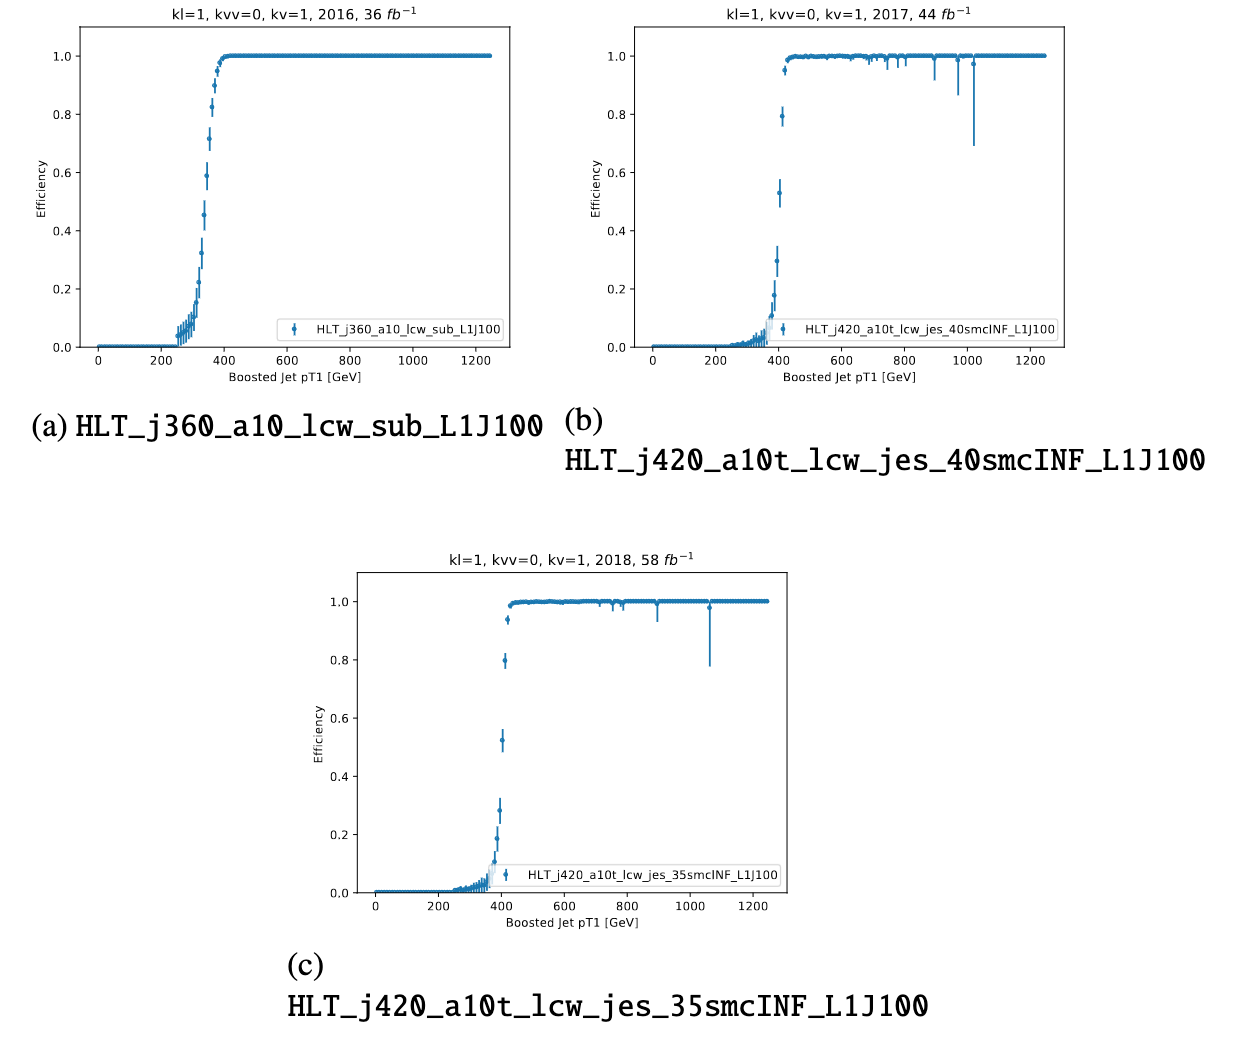
\includegraphics[width=1\textwidth]{trigger_eff}
%     \caption[]{{TODO MYSELF}}
%     \label{fig:trigger_eff}
% \end{figure}

\subsection{Large Radius Jets}
To fully capture the boosted Higgs pair topology, two \ac{ufo} large $R=1.0$ jets are selected as described in section \ref{sec:jets}. These jets are designed to enclose the two boosted collimated $b$-jets in each of them to form the Higgs candidates. If multiple large-$R$ jets are present, the two with the highest \pt are chosen. The large-$R$ jets are required to be within $200<p_{\text{T}}<2400$ GeV and $40<m<600$ GeV for which the jet calibration is valid. To ensure full efficiency for the trigger, the leading large-$R$ jet must have $\pt>\qty[]{450}{GeV}$.

The GN2X version of the $X\rightarrow bb$ tagger described in \ref{sec:gn2x} is used to identify large-$R$ jets containing two $b$-quarks. The calibration of this tagger starts from $\pt>\qty[]{250}{GeV}$ and is valid within the mass window $\qty[]{50}{GeV}<m<\qty[]{800}{GeV}$. Therefore, the subleading Higgs candidate is required to have $\pt>\qty[]{250}{GeV}$, and both Higgs candidates need to be within the mass window. The top fraction $f_\text{top}(f_\text{Hcc})$ is set to 0.25(0.02) and the \qty[]{60}{\percent} Higgs efficiency \ac{wp} is required. Higgs candidates must be non-overlapping, requiring $\Delta R(H_1, H_2) > 2.0$, though no overlap events were found.

\subsection{Small Radius Jets}
Two small radius $R=0.4$ jets are required for the \ac{vbf} signature and are referred to as \ac{vbf} jets in the following. They are reconstructed with the anti-$k_t$ algorithm and as \acp{pfo} described in \ref{sec:jets}. The tight \ac{wp} for the \ac{jvt} and the LooseBad \ac{wp} for the event cleaning are applied both described in \ref{sec:calibration}. Small-$R$ jets $j$ are selected for $\pt>\qty[]{20}{GeV}$ and $|\eta|<4.5$ for which the calibration is valid and are required to be outside of the Higgs candidate large-$R$ jets $J$ by imposing $\Delta R(J,j) > 1.4$.

It can be shown that the \ac{vbf} jets typically exhibit a large invariant mass for the ($j_1$, $j_2$) system and a significant pseudorapidity difference $|\Delta\eta(j_1,j_2)|$ \citep{rauch2016vectorboson}. Consequently, cuts are usually applied to these quantities in standard $HH\rightarrow 4b$ \ac{vbf} analyses. This analysis explores an automated optimization of these cuts, which will be discussed in chapter \ref{sec:analysis_optimization}.

\subsection{Kinematic Regions}\label{sec:kinematic_regions}
\ac{sr}, Validation Region (VR) and \ac{cr} are explored and optimized in previous analyses \citep{aad2023search,ATL-COM-PHYS-2023-033} in the $m_{H1},m_{H2}$ plane and are defined as
\begin{equation}
    SR =  \sqrt{\left(\frac{m_{H1} - \SI{124}{\GeV}}{1500 / m_{H1}}\right)^{2} + \left(\frac{m_{H2} - \SI{117}{\GeV}}{1900 / m_{H2}}\right)^{2}} < 1.6,
\end{equation}
\begin{equation}
    \label{VR_Xhh}
    VR =  \sqrt{\left(\frac{m_{H1} - \SI{124}{\GeV}}{0.1 \ln(m_{H1}/\text{GeV})}\right)^{2} + \left(\frac{m_{H2} - \SI{117}{\GeV}}{0.1 \ln(m_{H2}/\text{GeV})}\right)^{2}} < 100,
\end{equation}
and
\begin{equation}
    \label{CR_Xhh}
    CR = \sqrt{\left(\frac{m_{H1} - \SI{124}{\GeV}}{0.1 \ln(m_{H1}/\text{GeV})}\right)^{2} + \left(\frac{m_{H2} - \SI{117}{\GeV}}{0.1 \ln(m_{H2}/\text{GeV})}\right)^{2}} > 100  \ \& \ < 170.
\end{equation}
Figure \ref{fig:m_hh_plane} depicts $m_{H1}-m_{H2}$ planes for data and signal samples. As pointed out in the introduction of section \ref{sec:hh4b_analysis_strategy} here remains an opportunity for improvement.
\begin{figure}
    \centering
    % 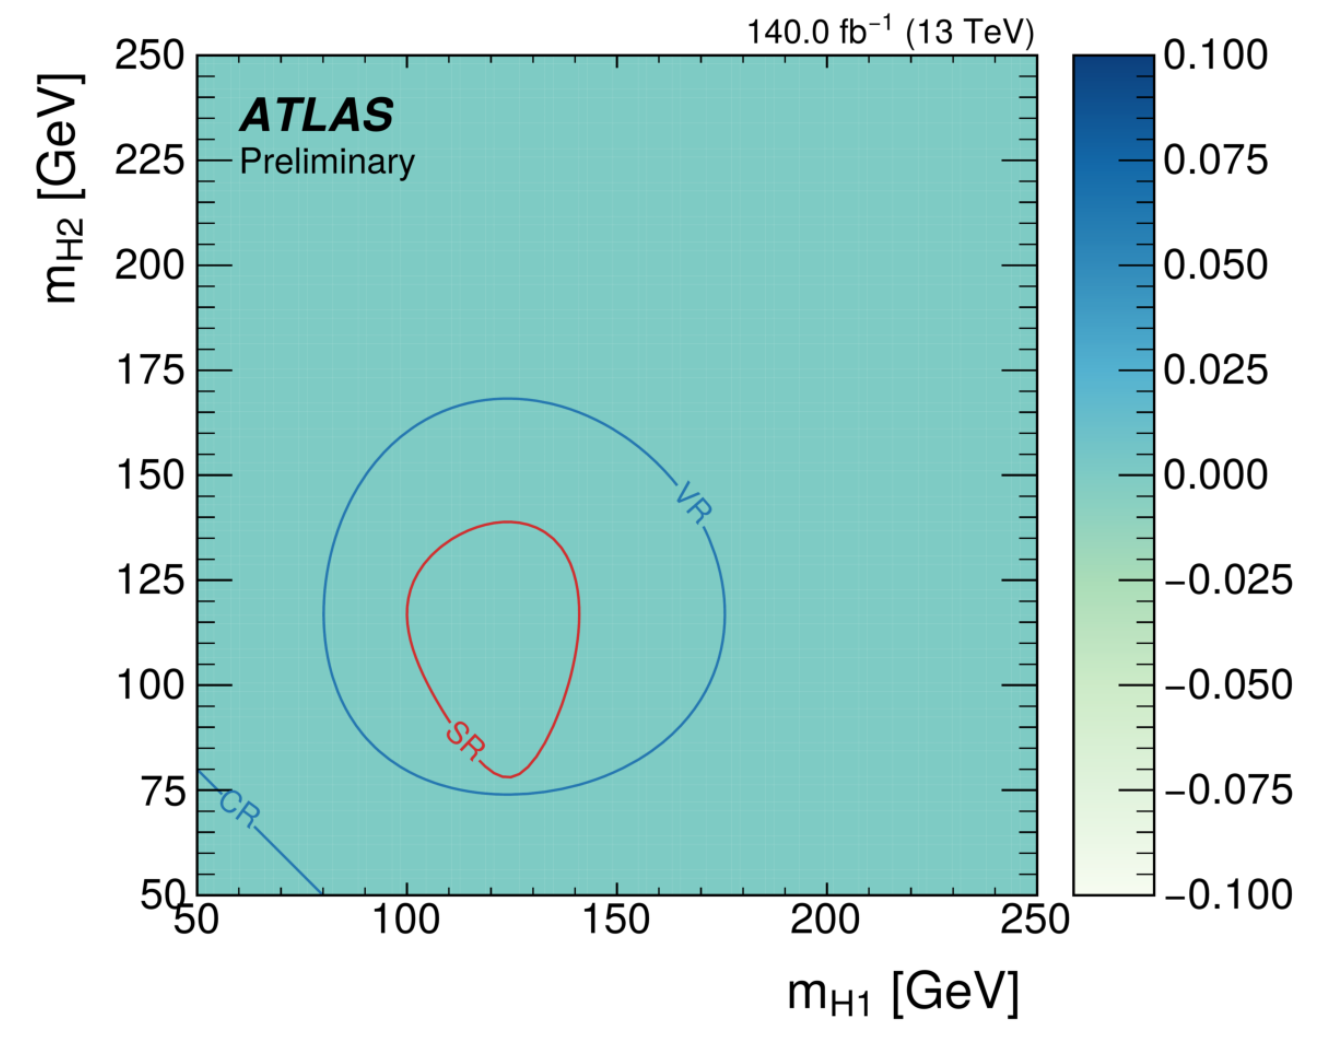
\includegraphics[width=.7\textwidth]{m_hh_plane}
    \subfigure[]{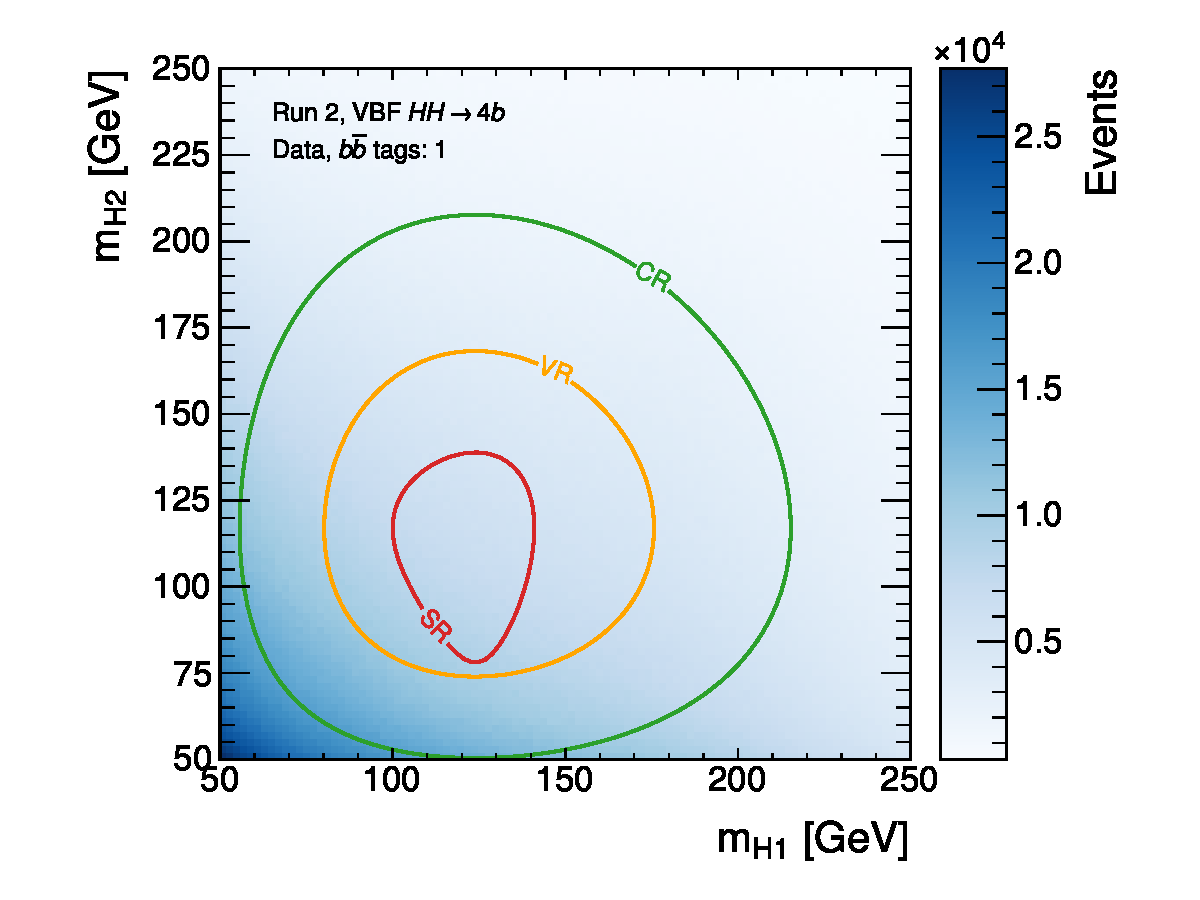
\includegraphics[width=.49\textwidth]{massplane_NOSYS.xbb_1_run2}}
    \subfigure[]{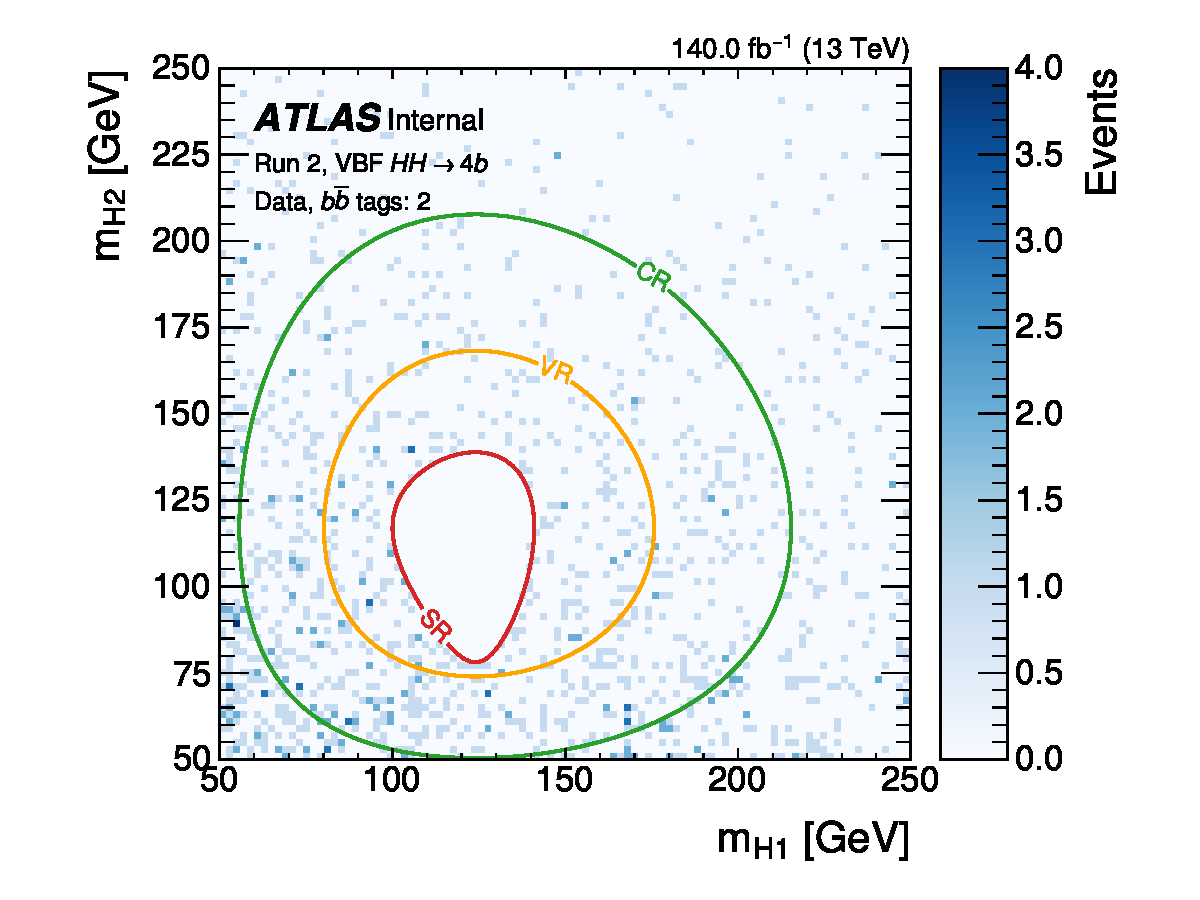
\includegraphics[width=.49\textwidth]{massplane_NOSYS.xbb_2_run2}}
    \subfigure[]{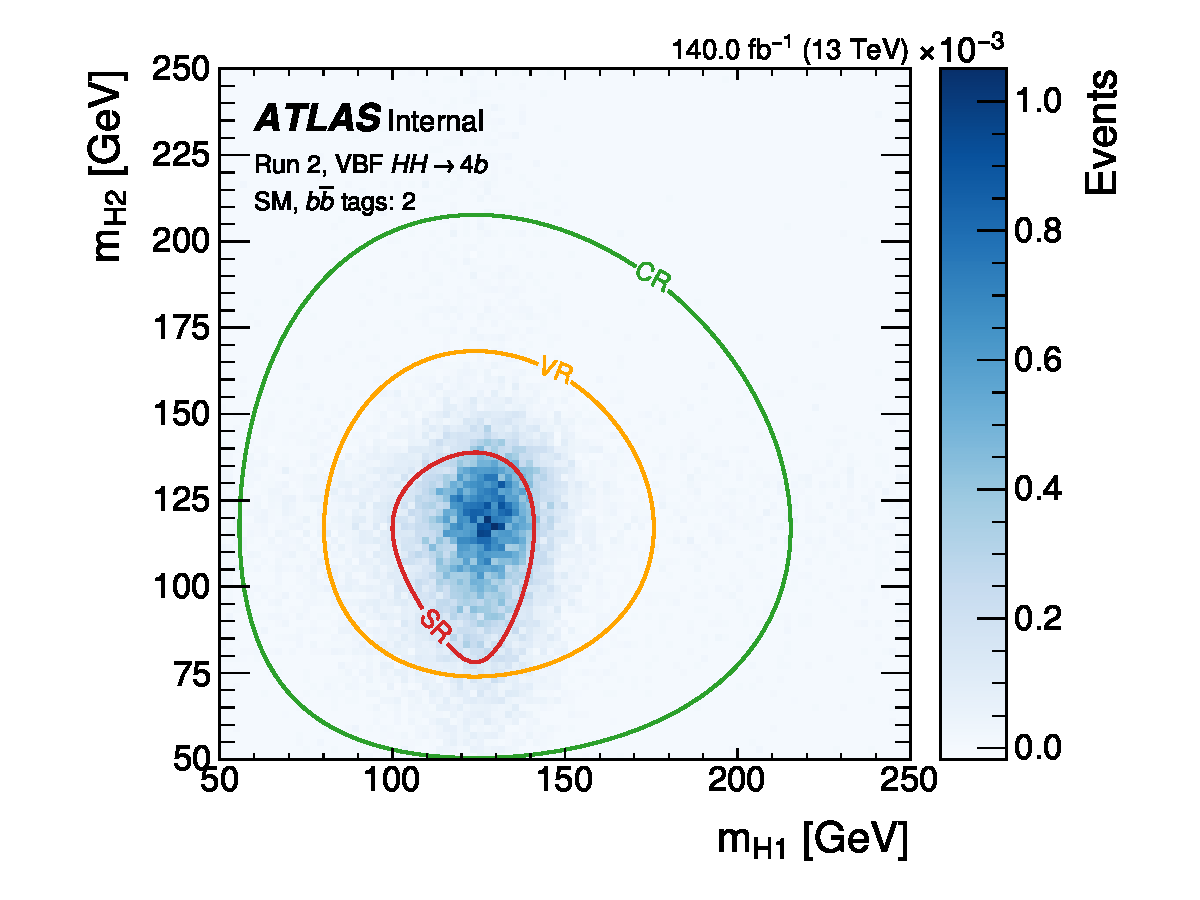
\includegraphics[width=.49\textwidth]{massplane_NOSYS.xbb_2_SM}}
    \subfigure[]{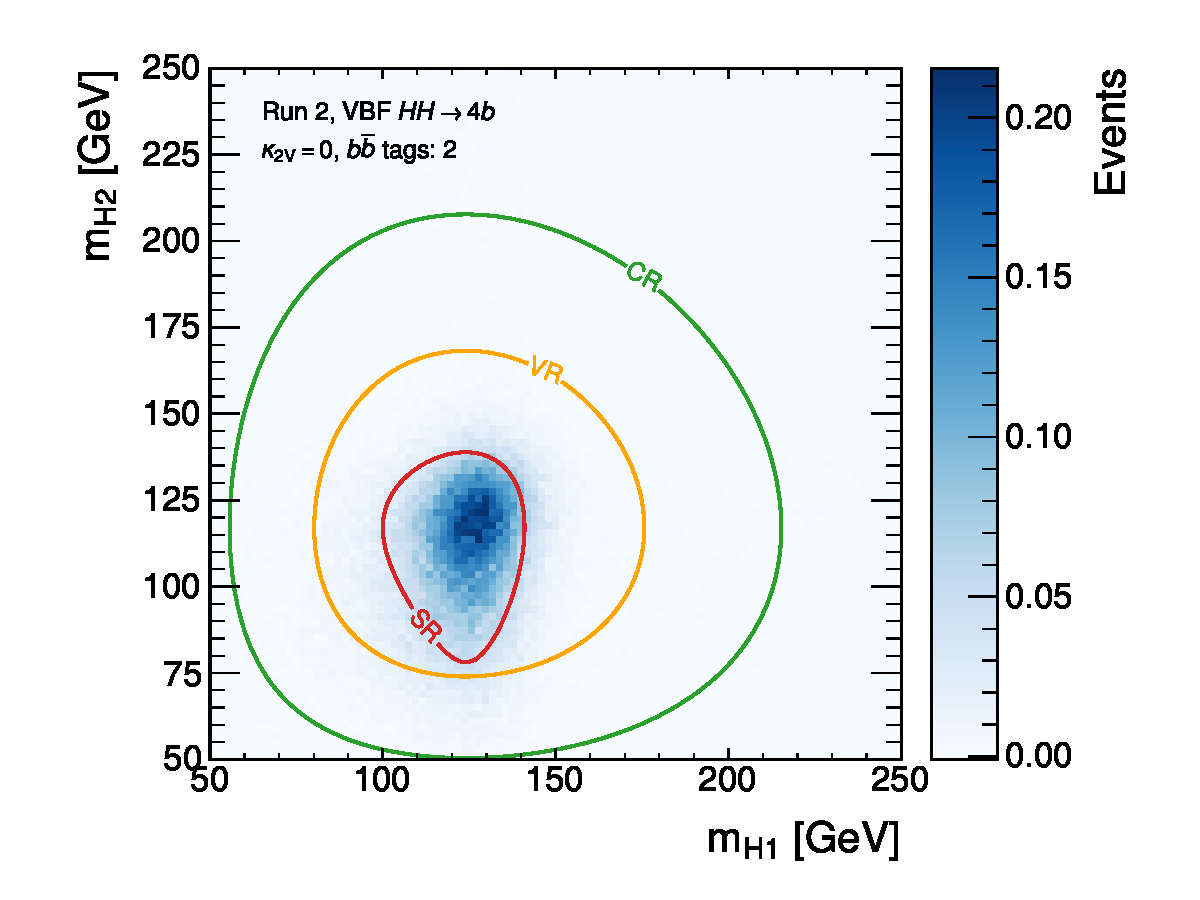
\includegraphics[width=.49\textwidth]{massplane_NOSYS.xbb_2_k2v0}}
    \caption[]{ $m_{H1}-m_{H2}$ planes after event selection for data with (a) 1 GN2X tag and (b) 2 GN2X tags, (c) a \ac{sm} and (d) $\ktwov$=0 signal sample with 2 GN2X tags. Defined kinematic regions are given as contours for \ac{cr}, \ac{vr} and \ac{sr}.}
    \label{fig:m_hh_plane}
\end{figure}

\subsection{Background Estimation}\label{sec:abcd}
Estimating the contributions from the various \ac{qcd} processes via simulation remains a significant challenge since hadrons constitute the final state in this analysis. Therefore, the ABCD method is employed to derive a data-driven background estimate \citep{buttinger2018background,PhysRevD.103.035021}. This method uses two independent variables, $f$ and $g$, to define four orthogonal regions: A, B, C, and D, as illustrated in Figure \ref{fig:abcd}, such that for a combination of event yield ratios in these regions, the following relationship holds:
\begin{equation}
    \frac{N_A}{N_B}=\frac{N_C}{N_D}.
\end{equation}
\begin{figure}
    \centering
    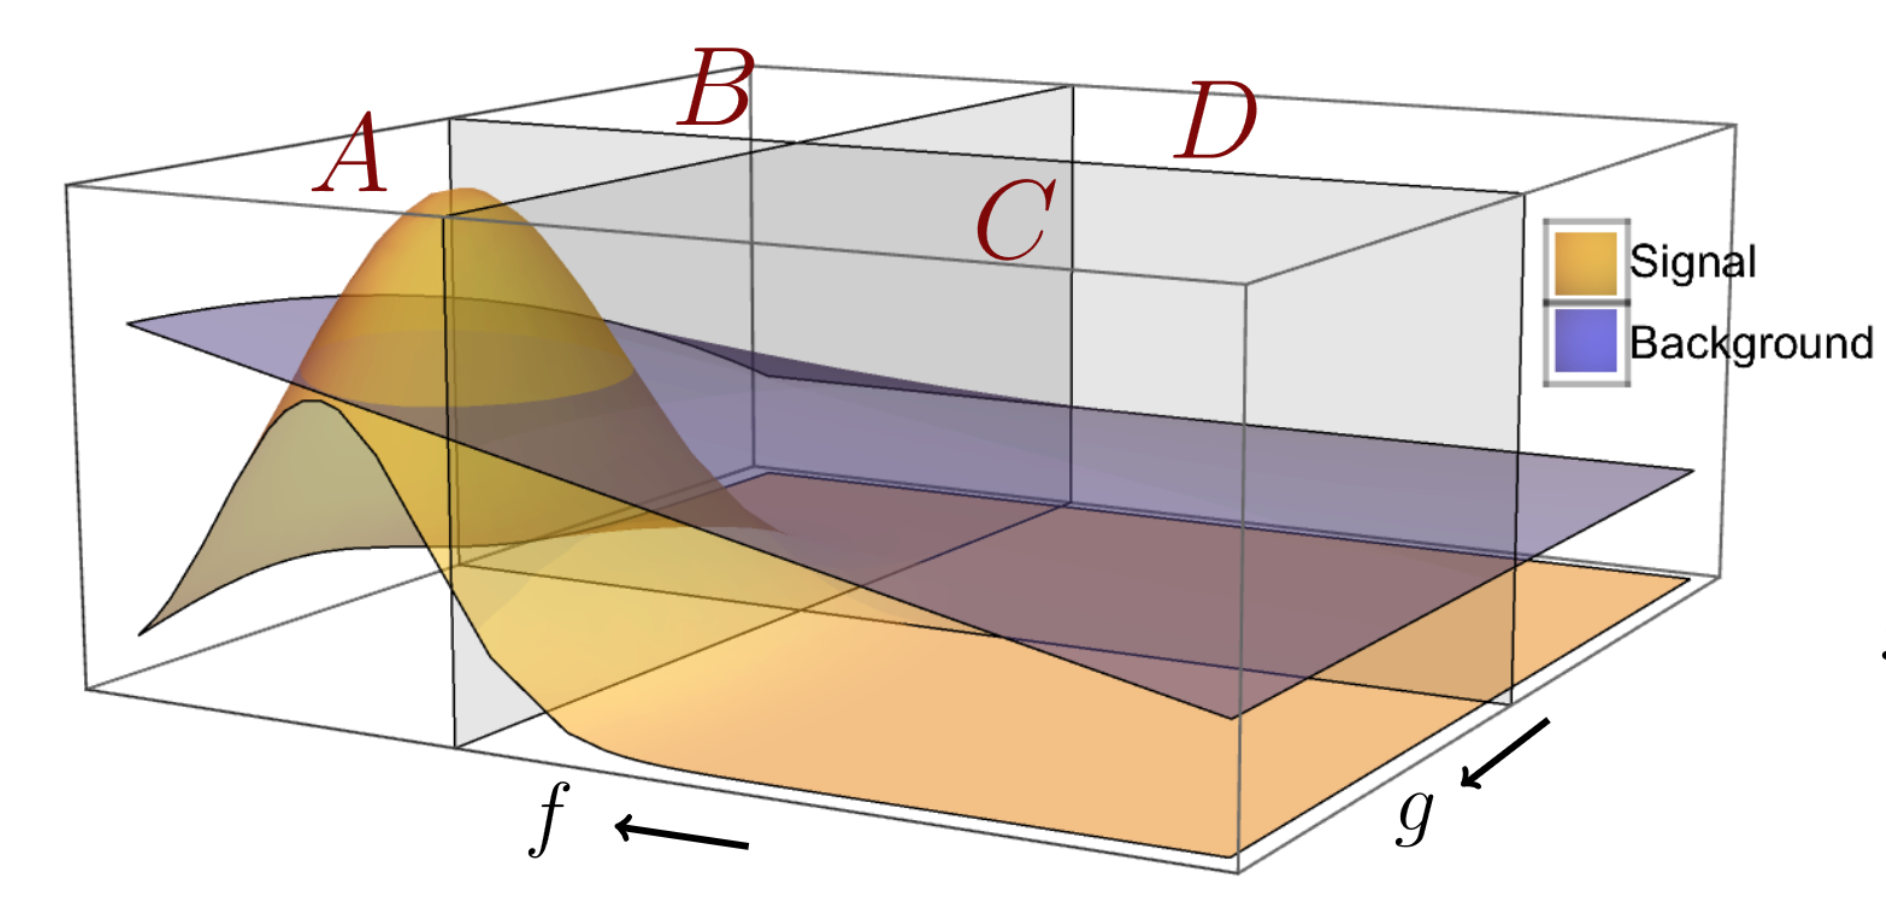
\includegraphics[width=.7\textwidth]{abcd}
    \caption[]{Illustration of four orthogonal regions A, B, C and D defined by two variables $f$ and $g$ in the horizontal and signal and background yields in the vertical dimension. Adopted from \citep{PhysRevD.103.035021}.}
    \label{fig:abcd}
\end{figure}
By rearranging the equation for the unknown $N_A$ an estimate for the background of the signal region can be derived from the other known yields that lie in the regions dominated by the background.

In this analysis the two orthogonal variables are defined via the amount of double-$b$ tagged large-$R$ jets with the GN2X tagger and the kinematic regions of the \ac{sr} and \ac{cr} defined in \ref{sec:kinematic_regions}.
\begin{table}[htbp]
    \centering
    \caption{Four orthogonal region definitions for the ABCD method}
    \begin{tabular}{|c|c|}
        \hline
        2 GN2X in CR & 2 GN2X in SR \\ \hline
        1 GN2X in CR & 1 GN2X in SR \\ \hline
    \end{tabular}
    \label{tab:abcd}
\end{table}
This gives the four orthogonal regions shown in table \ref{tab:abcd}. Hence, the background in the \ac{sr} is estimated with a weight extracted from the \ac{cr}
\begin{equation}
    N_\text{SR}^\text{2 GN2X}=\frac{N_\text{CR}^\text{2 GN2X}}{N_\text{CR}^\text{1 GN2X}} N_\text{SR}^\text{1 GN2X} = w_\text{CR} N_\text{SR}^\text{1 GN2X}=  (0.0038 \pm 0.0002) \times N_\text{SR}^\text{1 GN2X}.
\end{equation}

This approach relies on the assumption that the shape of the background in figure \ref{fig:abcd} does not vary greatly between C to D and A to B. To verify the robustness of this assumption variations between the expected and estimated region in the \ac{vr} are depicted in Figure \ref{fig:compareABCD}. The observed discrepancies are addressed by assigning an uncertainty to the background estimate, which is further detailed in Section \ref{sec:systematics}.
\begin{figure}
    \centering
    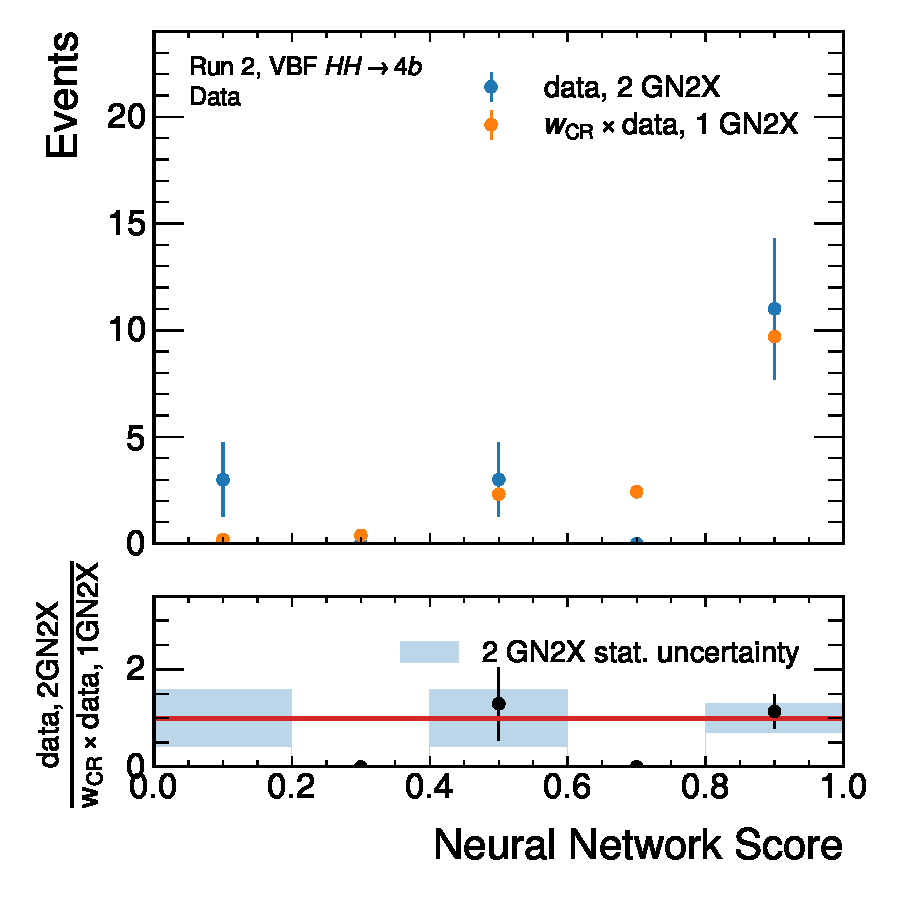
\includegraphics[width=0.7\textwidth]{tomatos_cls_5_2500_slope_50_NOSYS.VR_xbb_2_compareABCD.pdf}
    \caption[]{Comparison of \ac{nn} response in the \ac{vr} for the 2 GN2X tagged Higgs candidates and the background estimate from multiplying the 1 GN2X tagged selection with $w_\text{CR}$.}
    \label{fig:compareABCD}
\end{figure}

\subsection{Cutflow Analysis}
The cutflow tables are presented in the following order:

\begin{itemize}
    \item \textbf{Trigger:} Apply the trigger
    \item \textbf{Two fat jets:} Large-$R$ jet kinetic selection
    \item \textbf{Fat jet $\pt$:} Apply the $\pt > \qty[]{450}{GeV}$ cut after identifying the leading Higgs candidate
    \item \textbf{Two hbb jets:} Require 2 GN2X tags
    \item \textbf{VBF jets:} Find 2 small-$R$ jets compatible with the selection
    \item \textbf{VBF cut:} Apply cuts on $m_{j_1,j_2}$ and $|\Delta\eta(j_1,j_2)|$
    \item \textbf{SR:} Pass the signal region
\end{itemize}

\begin{table}[htbp]
    \centering
    \caption{Cutflow Run 2 data}
    \begin{tabular}{lrrr}
        \hline
        \textbf{Selection Step} & \textbf{Events}  & \textbf{Fraction (\%)} & \textbf{Cumulative (\%)} \\ \hline
        Initial events          & 1147720630.00000 & 100.00000              & 100.00000                \\\hline
        Trigger                 & 280935686.00000  & 24.47771               & 24.47771                 \\
        Two fat jets            & 72439244.00000   & 25.78499               & 6.31157                  \\
        Fat jet $\pt$           & 53743119.00000   & 74.19061               & 4.68260                  \\
        Two hbb jets            & 4089.00000       & 0.00761                & 0.00036                  \\
        VBF jets                & 1559.00000       & 38.12668               & 0.00014                  \\
        VBF cut                 & 201.00000        & 12.89288               & 0.00002                  \\
        SR                      & 0.00000          & 0.00000                & 0.00000                  \\\hline
    \end{tabular}
\end{table}

\begin{table}[htbp]
    \centering
    \caption{Cutflow $\kappa_\text{2V}=0$ signal}
    \begin{tabular}{lrrr}
        \hline
        \textbf{Selection Step} & \textbf{Events} & \textbf{Fraction (\%)} & \textbf{Cumulative (\%)} \\ \hline
        Initial events          & 1307.36934      & 100.00000              & 100.00000                \\\hline
        Trigger                 & 253.74720       & 19.40899               & 19.40899                 \\
        Two fat jets            & 180.06129       & 70.96090               & 13.77279                 \\
        Fat jet $\pt$           & 156.07723       & 86.68006               & 11.93827                 \\
        Two hbb jets            & 72.42898        & 46.40586               & 5.54006                  \\
        VBF jets                & 51.92269        & 71.68773               & 3.97154                  \\
        VBF cut                 & 40.37272        & 77.75545               & 3.08809                  \\
        SR                      & 28.03348        & 69.43668               & 2.14427                  \\\hline
    \end{tabular}
\end{table}



\begin{table}[htbp]
    \centering
    \caption{Cutflow \ac{sm} signal}
    \begin{tabular}{lrrr}
        \hline
        \textbf{Selection Step} & \textbf{Events} & \textbf{Fraction (\%)} & \textbf{Cumulative (\%)} \\ \hline
        Initial events          & 15.56347        & 100.00000              & 100.00000                \\\hline
        Trigger                 & 2.54380         & 16.34470               & 16.34470                 \\
        Two fat jets            & 1.15620         & 45.45160               & 7.42893                  \\
        Fat jet $\pt$           & 0.85139         & 73.63668               & 5.47041                  \\
        Two hbb jets            & 0.21498         & 25.25017               & 1.38129                  \\
        VBF jets                & 0.12550         & 58.37851               & 0.80638                  \\
        VBF cut                 & 0.07195         & 57.33242               & 0.46231                  \\
        SR                      & 0.04759         & 66.13817               & 0.30577                  \\\hline
    \end{tabular}
\end{table}









\subsection{Event Classification}\label{sec:event_classification}
A deep feed-forward neural network is employed for signal to background separation. This neural network's training uses a novel approach \textsc{neos}, which is discussed in detail in \ref{sec:analysis_optimization} alongside other \ac{ml} concepts.

Inputs to the neural network include 23 features, which are the four vector components ($\pt,\eta,\phi,m$) of: the Higgs boson pair system, the individual Higgs candidates and the two \ac{vbf} jets. In addition the leading score of the GN2X tagger and the mass of \ac{vbf} jet system $m_{j_1,j_2}$ and their pseudorapidity difference $|\Delta\eta(j_1,j_2)|$ are used. The \ac{nn} needs to be applicable across all samples, therefore only the leading GN2X score is incorporated, as the background estimation relies on a single GN2X tag.

The network's architecture features three fully connected layers, each comprising 100 nodes, and concludes with a singular output node. The hidden layers are followed by a rectified linear unit activation function whereas the output node employs a sigmoid activation for classification. The architecture is thus defined as [23,100,100,100,1], indicating the sequence of layers from input to output. Figure \ref{fig:nominal-hist} displays the nominal expected histogram for this analysis for several samples.

\begin{figure}
    \centering
    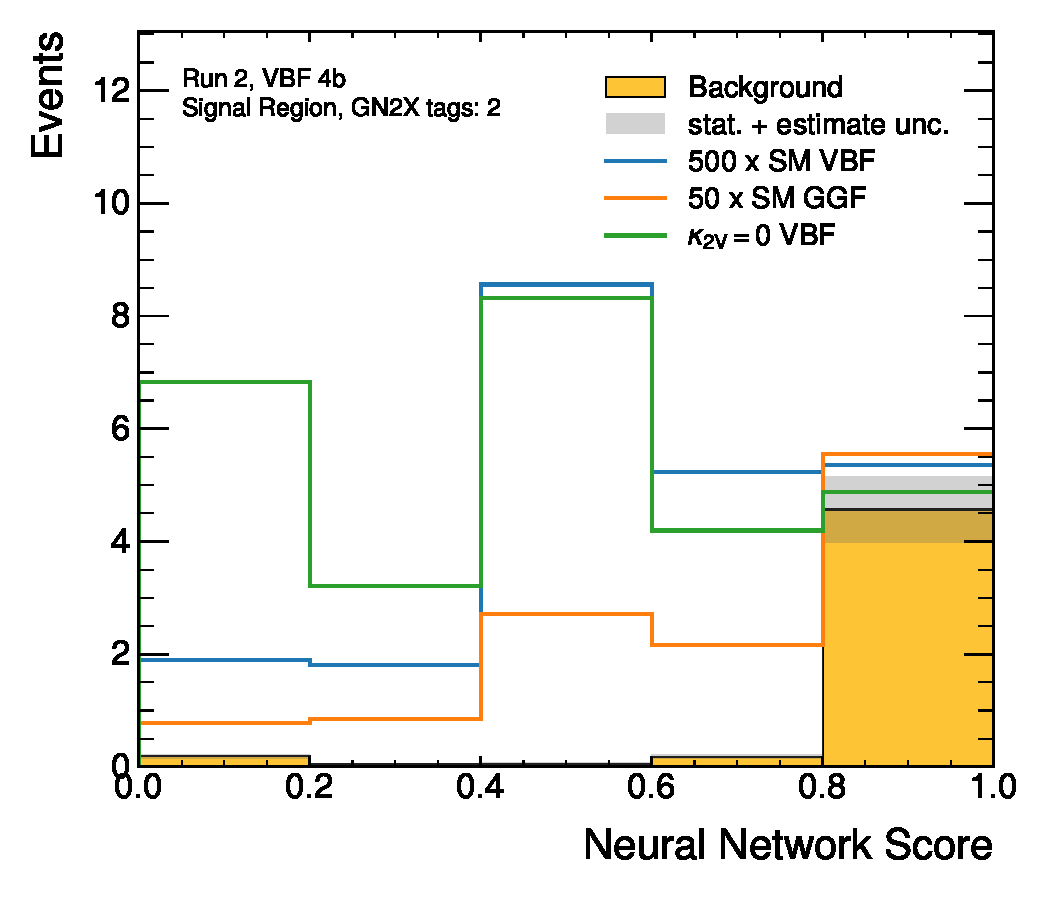
\includegraphics[width=0.7\textwidth]{tomatos_cls_5_2500_slope_50_NOSYS.SR_xbb_2_nominal_hist.pdf}
    \caption[]{\ac{nn} response for the data-driven background estimate, rescaled \ac{sm}  \ac{vbf} and \ac{ggf} signal and $\kappa_\text{2V}=0$.}
    \label{fig:nominal-hist}
\end{figure}


\section{Linear Combination of Signal Hypotheses}\label{sec:linear_combination}

This analysis is interested in constraining the couplings $\kappa_\text{V},\kappa_\lambda,\kappa_\text{2V}$ associated to the \ac{vbf} processes shown in figure \ref{fig:main_production_processes}. As computing resources are limited and MC generation is unfortunately computationally expensive only a few hypotheses are available. However by exploiting the properties of the differential cross-sectional calculation, samples of any hypothesized coupling value can be created through linear combination of samples \citep{ATLAS-CONF-2019-049}. Considering the \ac{vbf} diagrams of figure \ref{fig:main_production_processes} subscripted as (1,2,3) with couplings $\kl$, $\kv$ and \ktwov the differential (per bin) cross-section of a kinematic variable $x$, which can be e.g. the invariant mass of the Higgs pair system, can be rewritten as
\begin{align}
    \label{eqn:xsec_vbf}
    \frac{\mathrm{d}\sigma(\kvv, \kv, \kl )}{\mathrm{d} x } = &
    \left| A(\kvv, \kv, \kl ) \right|^2                                                                                               \\ \nonumber
    =                                                         & \left| \kv \kl M_1(x    ) + \kvv M_2(x  ) + \kv^2 M_3(x   ) \right|^2 \\ \nonumber
    =                                                         & \abs{M_1}^2 \kl^2 \kv^2  + 2 \mathcal{R}(M_{1}^* M_{2})  \kvv \kl \kv \\ \nonumber
                                                              & + 2 \mathcal{R}(M_{1}^* M_{3}) \kl \kv^3 + \abs{M_2}^2  \kvv^2        \\ \nonumber
                                                              & + 2 \mathcal{R}(M_{2}^* M_{3}) \kvv \kv^2 + \abs{M_3}^2 \kv^4.
\end{align}
The amplitude prefactors $M_i$ in front of the couplings depend non-trivially on $x$. However
rewriting equation \ref{eqn:xsec_vbf} by grouping the prefactors into $a_i$
\begin{align}\label{eq:reweight}
    \frac{\mathrm{d}\sigma(\kvv, \kv, \kl )}{\mathrm{d} x}
    = \; & a_1 \kl^2 \kv^2  + 2 a_2 \kvv \kl \kv  + 2 a_3 \kl \kv^3  \\
         & + a_4 \kvv^2     + 2 a_5 \kvv \kv^2 + a_6\kv^4, \nonumber
\end{align}
the equation depends on the couplings and the six prefactors. By plugging in six solutions of a bin content in the variable $x$, a system of equations can be solved to reduce the function to be solely dependent on $(\kvv, \kv, \kl )$ and deduce the cross-section for a desired hypothesis. Table \ref*{tab:vbf_hh_6term_varlist} shows the list of samples used for the derivation.
\begin{table}
    \centering
    \caption{6-Term VBF Combination Sample Variations}
    \label{tab:vbf_hh_6term_varlist}
    \begin{tabular}{ |l|l|l| }
        \hline
        \textbf {$\kappa_{2V}$} & \textbf {$\kappa_\lambda$} & \textbf {$\kappa_V$} \\
        \hline
        1                       & 1                          & 1                    \\
        1.5                     & 1                          & 1                    \\
        1                       & 2                          & 1                    \\
        1                       & 10                         & 1                    \\
        1                       & 1                          & 0.5                  \\
        1                       & -5                         & 0.5                  \\
        \hline
    \end{tabular}
\end{table}
The approach is employed bin-wise as the extraction factors can deviate substantially per bin as shown in figure \ref{fig:linear_combine_bin_solutions}.
\begin{figure}
    \centering
    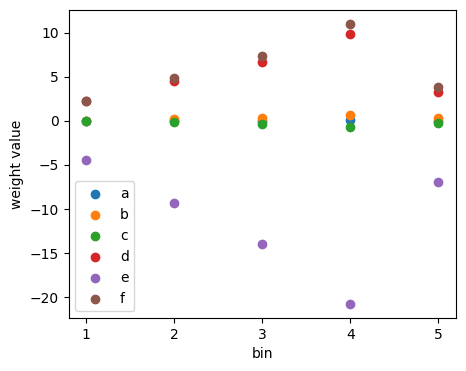
\includegraphics[width=.47\textwidth]{linear_combine_bin_solutions}
    \caption[]{Extracted reweighting factors per bin for equation \ref{eq:reweight}.}
    \label{fig:linear_combine_bin_solutions}
\end{figure}
The method is tested on the mc generated $\ktwov=0$ sample. Figure \ref{fig:tomatos_cls_5_nominal_reweighted_ratio} reveals a up to $\sim$\qty[]{16}{\percent} deviation for this approach. However the difference on cross-section limits determined with the mc generated $\ktwov=0$ and a reweighted $\ktwov=0$ signal is $\sim\qty[]{3}{\percent}$. It is further noted that this approach possibly suffers also from a sample choice which only explores the phase space for two $\ktwov$ couplings.
\begin{figure}
    \centering
    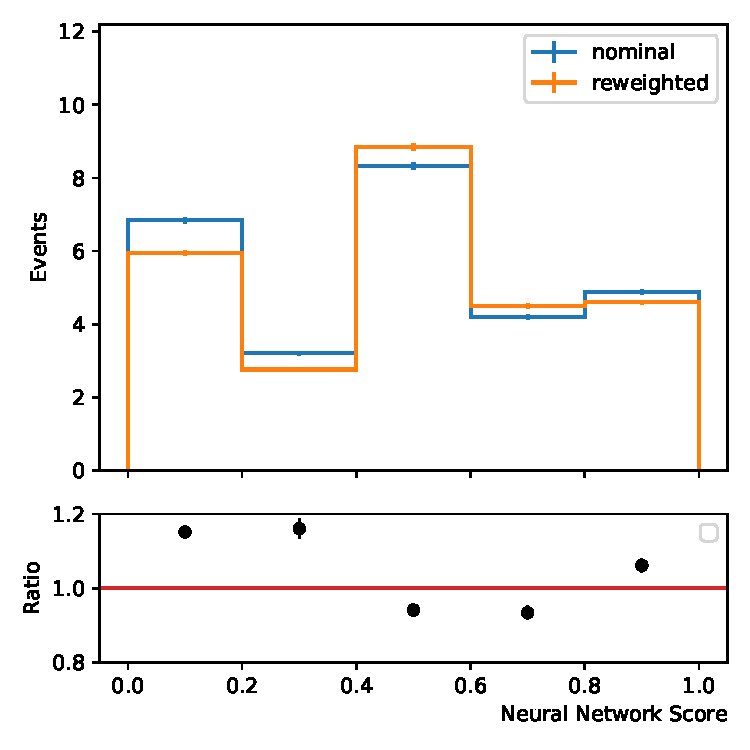
\includegraphics[width=.6\textwidth]{tomatos_cls_5_2500_slope_50_nominal_reweighted_ratio.pdf}
    \caption[]{Comparison between a \ac{mc}-generated $\ktwov=0$ signal sample and a signal sample created with the reweighting approach by linearly combining different \ktwov hypotheses. }
    \label{fig:tomatos_cls_5_nominal_reweighted_ratio}
\end{figure}


% , another one would be  
% l0cvv1cv1, however why validating for kl if we scan k2v, I don't think this validation is worth anything in a phase space we are not testing on.



% https://www.overleaf.com/project/638e1930f926cd21d5264259
% https://trexfitter-docs.web.cern.ch/trexfitter-docs/model_building/expression/
% https://gitlab.cern.ch/hh4b/hh4b-boosted-vbf-limits/-/blob/main/create_workspaces/configs/k2V_parameterized_BDT_decorXbb.config?ref_type=heads#L285-331

